
% \section{Data-Driven Hypotheses and Hypothesis Semantic Trees}
\section{Formalization}
% \section{Preliminaries}% \section{Background}
\label{sec:background}

We begin by formalizing what we mean by a data-driven hypothesis and how the structure of a complex hypothesis may be viewed as a hypothesis semantic tree.

% \newpara{Data-Driven Hypothesis.}
A \textbf{data-driven hypothesis} $h$ in $\mathcal{H}$ (the space of such hypotheses) is a declarative sentence about the state of the world whose truth value may be inferred from a given dataset $D$ using a verification procedure $\mathcal{V}_D:\mathcal{H} \to \{\mathrm{supported}, \mathrm{unsupported}\}$, for instance, via statistical modeling. 
% \pete{Is true/false too black-and-white? In some cases we infer truth but more often we infer something less certain, e.g., X and Y are somewhat linearly correlated, gender somewhat predicts survival on the Titanic, etc.  I guess we can fold any uncertainty into the hypothesis itself, e.g., "Is it {\it true} that gender {\it somewhat} predicts survival?"....}
% \bodhi{the binary nature may be attributed to the fact that this verification process is grounded in a specific dataset?} \ashish{Even so, I think statistically speaking, given a dataset $D$, one can say that $h$ is supported by $D$ (with high confidence, p-value, etc.), $h$ is rejected by $D$ (again with high confidence), or $D$ neither supports nor rejects $h$ in a statistically significant way. Is it the case that the ``false'' here is clubbing the latter two, i.e., that $D$ does not support $h$ strongly enough (which is different from claiming that $h$ is false)?} \ashish{If true, you could replace `true' / `false' with something like `supported' / `unsupported'.} \bodhi{this is good: we can switch to this nomenclature}

% \newpara{Sub-hypothesis.}
Each hypothesis may further be expressed using a propositional formula $\phi$ over a set of \textbf{sub-hypotheses} $h_i \in \mathcal{H}$ using logical connectives, e.g., disjunctions and conjunctions, such that $h := \phi(h_1, \ldots, h_n)$ and $\mathcal{V}_D(h)=\phi(\mathcal{V}_D(h_1),\ldots,\mathcal{V}_D(h_n))$. For instance, suppose $h$ is the hypothesis \textit{``for men younger than 20, popularity of product A varies proportional to their age \textbf{($h_1$)}, while there exists an inverse relationship for those older than 40 \textbf{($h_2$)}''}, then $h$ can be expressed as the conjunction $h_1 \wedge h_2$.

% \newpara{Hypothesis Dimensions.}
Inspired by recent work of \citet{thompson2023scope}, we additionally introduce a structured formalism that breaks a hypothesis down into \textbf{three hypothesis dimensions}:
% \begin{itemize}[left=2pt, itemsep=0.1pt]
\begin{ite}
    \item \textbf{Contexts $(c)$:} Boundary conditions that limit the scope of a hypothesis.
    % \footnote{It is also possible to not specify the context, in which case the assertion in the hypothesis is unbounded.}
    E.g., \textit{``for men over the age of 30''} or \textit{``in Asia and Europe''} or unbounded/full dataset when not specified.
    \item \textbf{Variables $(v)$:} Known set of 
    % independent and dependent 
    concepts that interact in a meaningful way under a given context to produce the hypothesis. E.g., \texttt{gender}, \texttt{age}, or \texttt{income}. Note that each hypothesis is associated with a target variable and a set of independent variables.
    % Note that known concepts may either be independent variables or previously derived hypotheses.
    \item \textbf{Relationships $(r)$:} Interactions between a given set of variables under a given context that produces the hypothesis. E.g., \textit{``quadratic relationship''}, \textit{``inversely proportional''}, or piecewise conditionals.
\end{ite}
% Using these, we can now define a hypothesis as $c \wedge (\wedge_i^n vr^{(i)})$, where $vr^{(i)}$ is the $i$th variables-relationship pair in $h$. 
With slight abuse of notation, we can now equivalently define hypothesis $h:= \psi(c, v, r)$, where $\psi(\cdot,\cdot,\cdot)$ returns the declarative sentence
% ``relationships $r$ exist between variables $v$ under context $c$''.
\textit{``under context $c$, variables $v$ have relationship $r$.''}
For instance, for sub-hypothesis $h_1$ in our example above, $c_1 :=$ \textit{``men younger than 20''}, $v_1 :=$ \{\texttt{gender}, \texttt{consumer\_age}, \texttt{product\_popularity}\}, and $r_1 := 
 $\textit{``popularity is proportional to age''}.
% \ashish{At this point (or just before this sentence), would be helpful to spell out what exactly are $c, v,$ and $r$ in the example hypothesis above about product popularity}

% $(c, \{vr_i\}_{i=1:n})$, where $\mathbf{vr_i}$ is the $i$th variables-relationship interaction found in the hypothesis. Intuitively, this says that hypothesis $h$ asserts that there exist $n$ relationships between subsets of $v$ amongst variables $v$ under context $c$.
% where $c$ and $vr$ are boolean dimension-membership functions for contexts\footnote{It is also possible to not specify the context, in which case $c(\cdot)$ always evaluates to true.} and variable-relationship\footnote{Note that variables and relationships are only meaningful in conjunction, therefore we take a joint treatment of these dimensions, e.g. ``\texttt{age} is \emph{inversely proportional} to \texttt{travel frequency}''.} pairs, respectively.

\newcommand{\hyptree}{\mathcal{T}_h}
\newcommand{\hypsubtree}{\mathcal{T}_{h'}}

\begin{wrapfigure}[16]{r}{0.45\textwidth}
  \centering
  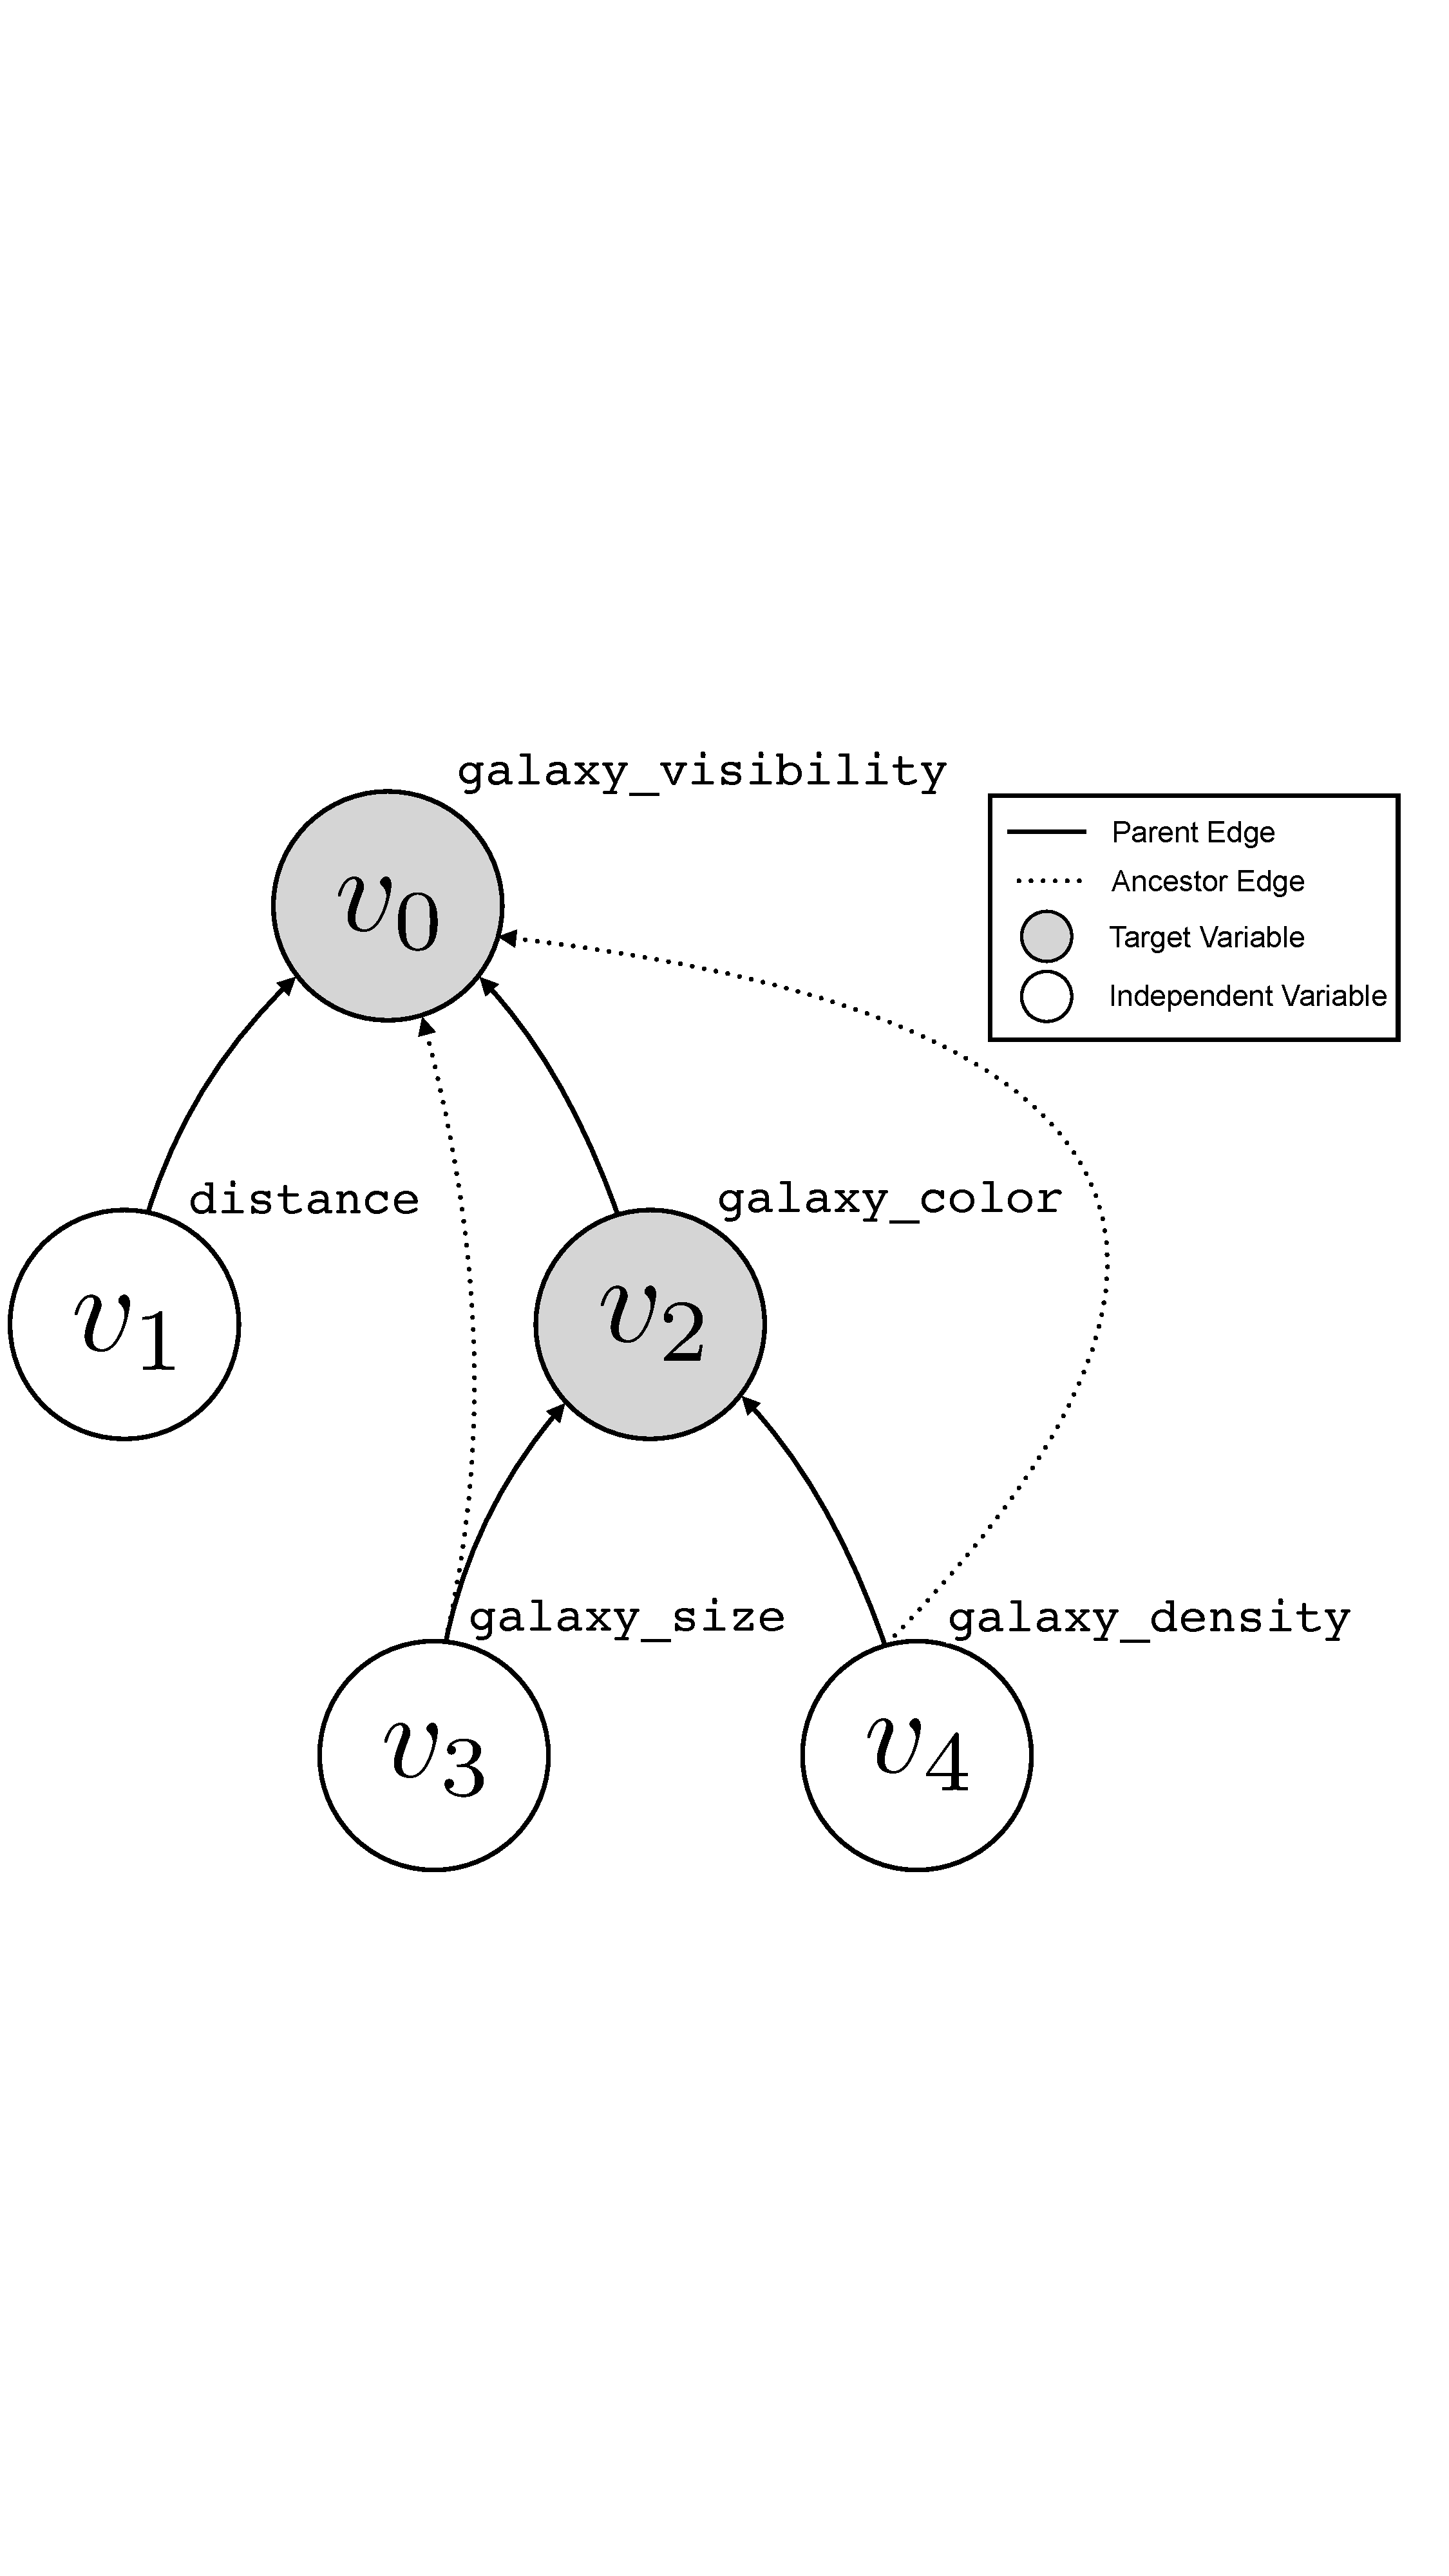
\includegraphics[trim=0 0 0 0, clip, width=0.9\linewidth]{figures/semantic_tree.pdf}
  \caption{Hypothesis Semantic Tree}
  \label{fig:semantic_tree}
\end{wrapfigure}
\newpara{Hypothesis Semantic Tree.}
Observe that each independent variable in a hypothesis may itself be a target variable for a prior hypothesis.
To emphasize this hierarchical nature, we introduce the concept of a \emph{hypothesis semantic tree} whose nodes are variables (independent or derived) and whose sub-trees represent hypotheses, as follows. Consider a hypothesis $h$. 
A semantic hypothesis tree $\hyptree$ with $h$ as the \emph{primary} hypothesis is a Markov tree whose root node is the target variable of $h$, each of whose leaf nodes is an independent variable that is not derived further, and each of whose internal nodes is the target variable of an \emph{intermediate} hypothesis.
In other words, each sub-tree $\hypsubtree$ rooted at an internal node $v$ of $\hyptree$ is itself a hypothesis semantic tree for a hypothesis $h'$ with $v$ as the target variable. 
In particular, a sub-tree rooted at $v$ and all its immediate children $C_v$ implicitly encodes $h'$ as $\psi(c, \{v\} \cup C_v, r)$ where $r$ is the relationship between $v$ and $C_v$
under context $c$ as specified in $h'$.
% , and $c$ is the context (??? context of $h$ or something else?). 
More generally, $\hyptree$ can encode many different hypotheses by choosing one node as the target variable and considering nodes at arbitrary descendant levels as independent variables.
% In general, a sub-hypothesis may be formed in multiple ways from $\hyptree$ by choosing one node as the target node and considering some subset of its descendants as independent variables (not sure if this is true or useful).
% Don't think we need the below (not used in subsequent sections):
% We also define $\texttt{depth}(\cdot)$ and $\texttt{height}(\cdot)$ of a node as measuring the maximum path lengths of the node to the root and from the leaves of $\mathcal{T}$, respectively.

For instance, in Fig~\ref{fig:semantic_tree}, we show a semantic tree $\hyptree$ with the following primary hypothesis ($h$): \textit{``The visibility of a galaxy reduces when the blue spectrum dominates and the distance of the galaxy from Earth increases''}, where \texttt{galaxy\_visibility} ($v_0$) is the target variable with independent variables \texttt{distance} ($v_1$) and \texttt{galaxy\_color} ($v_2$). Consider now the sub-tree rooted at $v_2$, which encodes the following intermediate hypothesis: \textit{``Visibility of blue light from galaxies increases with an increase in galaxy size and decrease in star density''}, where \texttt{galaxy\_color} ($v_2$) is the target variable with independent variables \texttt{galaxy\_size} ($v_3$) and \texttt{galaxy\_density} ($v_4$). Note further that due to there existing ancestor edges from $v_3$ and $v_4$ to $v_0$, $\hyptree$ also encodes the hypothesis: \textit{``The visibility of a galaxy reduces with distance from Earth combined with an increase in galaxy size and decrease in star density''}, where the target variable is $v_0$ and the independent variables are $v_3$ and $v_4$.

% % of hypotheses, 
% % \ashish{non-leaf node?}\dhruv{this should be leaf node; added} 
% % in $\mathcal{T}_h$ can recursively be split 
% % \ashish{this is confusing, I think. Instead of talking in terms of splitting a node etc.\ (which is about the \emph{process} of tree construction), for concept definition purposes, it would be better to talk about what the tree $\mathcal{T}_h$ contains \emph{after} it has been constructed: the root node of $\mathcal{T}_h$ corresponds to the target variable of $h$, the leaves of $\mathcal{T}_h$ correspond to ..., intermediate nodes to ..., hypothesis $h$ corresponds to ..., sub-hypotheses correspond to ..., etc.}
% using an intermediate hypothesis into new independent variables as child nodes. Each child node has a directed edge going to its parent (target variable), which implicitly encodes the hypothesis $\psi(c,v,r)$ \ashish{need something like: where $v$ consists of the parent along with all its children, $r$ is the relationship between the parent and its children, and $c$ is (???)}. For instance, as shown in Figure~\ref{fig:semantic_tree}, the hypothesis from our earlier example would have $\texttt{product\_popularity}$ as the root variable $h$ in the tree with $\texttt{consumer\_age}$ and $\texttt{gender}$ as its child nodes. Then, $\texttt{consumer\_age}$ may further be split into $\texttt{price\_preference}$ and $\texttt{color\_preference}$ given an intermediate hypothesis that asserts that ``older customers tend to buy more expensive products with a milder hue''.
% The resulting structure is a directed acyclic graph \ashish{if it's allowed to be a DAG in general, should we rename hyp.~semantic tree to hyp.~semantic graph? alternatively, if in practice you (almost-)always construct trees, it's better to stick to trees everywhere and just add a footnote that one may generalize this to DAGs}, % anti-arborescence
% where independent variables are always the leaves, 
% the root variable corresponds to a \emph{primary} hypothesis, and internal nodes represent derived variables corresponding to \emph{intermediate} hypotheses. \tushar{Should we give an example of the hypothesis for h given v1, v3, v4? This will also help ground task complexity?} \ashish{as we discussed, looks like this may not be easy for this particular example. Can we switch to a different example where this is easier to illustrate?}
% % Note that semantic trees rooted at independent variables are always isolated nodes. 
% We also define $\texttt{depth}(\cdot)$ and $\texttt{height}(\cdot)$ of a node as measuring the maximum path lengths of the node to the root and from the leaves of $\mathcal{T}$, respectively. 

% \harshit{It will help immensely if we connect the Hypothesis Semantic Tree to the real-world benchmark as well because concepts like height and depth cannot be defined there and we do not talk about them. Hypothesis definition and dimensions connect to the real world and we cover the examples, so this will complete the picture.} \dhruv{To be able to use the tree in real, one way is to say that knowing the tree structure from a given dataset a priori is hard/impossible because of incomplete information about unobserved intermediate nodes and no knowledge of edges between observed nodes from just a dataset. Then, (and Bodhi had this point), we say: however, workflow can be a proxy for the path length between target and leaves, controlling the task difficulty.}


\newpara{(Task) Dataset.} We formally define a dataset $D$ on which hypothesis search and verification is performed as a collection of tuples $\{\mathbf{x}_i\}_{i=1}^m$ that 
% encodes a 
% disjoint 
% union of 
% \ashish{`encoding a union of multiple hypothesis trees' sounds odd for a dataset. How about simply `supports multiple ...'?} 
supports
multiple hypothesis semantic trees
resulting in a \textit{semantic forest} $\mathcal{F}:=\cup_i\mathcal{T}_{h^{(i)}}$, where each $\mathbf{x}_i$ is a row in the dataset and $x \in \mathbf{x}_i$ is an observation for a particular column. Further, $\mathbf{x}_i$ may span only a subset of nodes in $\mathcal{F}$, i.e., not all nodes in $\mathcal{F}$ may be observed. 
Specifically, while roots and leaves are always observed, internal nodes (target variables for intermediate hypotheses) may be latent.
Therefore, multiple versions of $D$ may be collected for $\mathcal{F}$ with different degrees of observability of internal nodes, altering the difficulty of the discovery task.
% For instance, a tree in $\mathcal{F}$ with a large depth may contain several intermediate hypotheses that have not explicitly been collected as observations in the dataset.
% For instance, in the presence of multicollinearity in a dataset, an intermediate hypothesis in $\mathcal{F}$ would be observed along with its child nodes. 
% On the other hand, a tree in $\mathcal{F}$ with a large depth (i.e. a complex primary hypothesis) may contain several unobserved intermediate hypotheses. 
% A corollary of the previous statement is that multiple datasets may be constructed from $\mathcal{F}$ varying the observability of intermediate nodes, thus altering the difficulty of the hypothesis discovery task.

% \paragraph{Pipeline.} Note further that each observation $\mathbf{x}_i \in D$ may contain some noise due to common data collection challenges, e.g., human error, sampling bias, inconsistent standards, or instrument errors. \dhruv{Unclear how we plan to use "pipeline" subsequently. Will revisit once we have clarity on that.}

% \bodhi{need some transition to the next section}






%%%%%%%%%%%% GRAVEYARD %%%%%%%%%%%%%%

% \section{Background}
% \label{sec:background}
% \paragraph{Scope-based View.}We first provide a formalism for a \emph{hypothesis} that takes a set-theoretic view based on a notion of \emph{hypothesis scope} \citep{thompson2023scope}. 
% Let hypothesis $H := \{s_i\}$ be the set of permissible situations that allow the hypothesis to be accepted.
% Each situation $s \in \mathcal{S}$ represents a possible state of the world for which the truth value may be inferred using a dataset $D \in \mathcal{D}$ with a hypothesis verification procedure $\mathcal{V}_H : \mathcal{S} \times \mathcal{D} \rightarrow \{\mathrm{true}, \mathrm{false}\}$ (e.g., via statistical modeling, symbolic regression, etc.). 
% Therefore, $H$ is only accepted if $\exists s \in H,D \in \mathcal{D}$ s.t. $\mathcal{V}_H(s,D)$. \dhruv{Edit to contextualize with only the given dataset.}
% As $|H|$ increases, the number of situations that may result in the hypothesis being accepted increases, i.e. the hypothesis becomes \emph{broad} (conversely, as $|H|$ decreases, the hypothesis becomes \emph{narrow}).

% \paragraph{Set Membership.} However, enumerating all situations encoded by a hypothesis may be intractable (e.g., ``there exists a linear relationship between $x$ and $y$'' results in an uncountable set). We, therefore, formulate an alternative definition that is based on set membership functions.
% Let $\mathcal{M}_{H}: \mathcal{S} \rightarrow \{\mathrm{true}, \mathrm{false}\} := \vee_{i=1}^n~h_i(s)$ be a boolean membership function expressed in disjunctive normal form (DNF) \dhruv{Change to conjunction; could add a footnote saying disjunction is possible as well} over $n$ sub-hypotheses $h_i$ ($n \ge 1$) such that $H = \{s~\vert~ s \in \mathcal{S} : \mathcal{M}_H(s)\}$. Each term $h_i$ in $\mathcal{M}_H$ is also a boolean function, which we parameterize using three dimensions---\emph{contexts}, \emph{variables}, and \textit{relationships}---defined as follows:

% \begin{itemize}[left=2pt, itemsep=0.1pt]
%     \item \textbf{Contexts $(c)$:} Boundary conditions that limit the scope\dhruv{use different word} of a sub-hypothesis. E.g., ``for men over the age of 30'', ``in Asia and Europe''.
%     \item \textbf{Variables $(v)$:} Known concepts that interact in a meaningful way under a given context to produce the sub-hypothesis. E.g., \texttt{gender}, \texttt{age}, \texttt{income}. Note that known concepts may either be independent variables or previously derived hypotheses.
%     \item \textbf{Relationships $(r)$:} Interactions between a given set of variables under a given context to produce the sub-hypothesis. E.g., ``quadratic relationship'', ``inversely proportional'', piecewise conditionals.
% \end{itemize}

% Formally, we can now define the sub-hypothesis membership function $h_i(\cdot) := (c_i(\cdot) \wedge vr_i(\cdot))$, where $c_i(\cdot)$ and $vr_i(\cdot)$ are boolean dimension-membership functions for contexts\footnote{It is also possible to not specify the context, in which case $c(\cdot)$ always evaluates to true.} and variable-relationship\footnote{Note that variables and relationships are only meaningful in conjunction, therefore we take a joint treatment of these dimensions, e.g. ``\texttt{age} is \emph{inversely proportional} to \texttt{travel frequency}''.} pairs, respectively. For the rest of this work, we use our DNF-based definition $\mathcal{M}_H$ for a hypothesis and readout $\mathcal{R}(\mathcal{M}_H)$ to express it in natural language.



% % \harshit{should we also add the pipelines definition that Ashish suggested here? Pipelines (P) - function (Data, Hypothesis) Possible configurations of data transformations over XY. E.g., derive variables (“5x1.x2”), drop unreliable observations, standardizing, correcting confounding variables
% % Deterministic transformation, clean-up, …
% % }
% % \bodhi{pipeline can appear after Query Dataset is defined and can say that the pipeline is used to construct the semantic starting from leaf nodes -- this involves both hypothesis search and verification at each level}
% % \dhruv{I was thinking about this. I had deliberately left it out in the initial draft because pipeline is closely tied in with the dataset, and seems to me as quite distinct a concept from context, variables, and relationships. I'm not sure if it fits well in defining the semantic tree construction either -- you need pipeline to \textit{find} the path in the tree, but not necessarily to define the tree.}
% % \bodhi{I agree, then simply we could add it after the Query Dataset is defined.}
% % \harshit{understood, makes sense}

% \paragraph{Hypothesis Semantic Tree.} To emphasize the hierarchical nature of hypotheses, where interacting variables may themselves be prior hypotheses, we introduce the concept of a \emph{semantic tree}. Let $\mathcal{T}(\mathcal{M}_H)$ be a Markov tree rooted at $H$, where each node can recursively be split into its interacting variables $v \in \{vr_i\}_{i=1}^n$ as child nodes with the edges going into the parent node jointly encoding $\mathcal{M}_H$. The resulting structure is an anti-arborescence, where independent variables are always the leaves, 
% the root represents a \emph{primary} hypothesis, and internal nodes represent derived variables or \emph{intermediate} hypotheses.
% Note that semantic trees rooted at independent variables are always isolated nodes. We also define $\texttt{depth}(\cdot)$ and $\texttt{height}(\cdot)$ for a node in a tree as measuring the maximum path lengths of the node to the root and from the leaves of $\mathcal{T}$, respectively.

% \paragraph{Task Dataset.} We now define a dataset $D$, on which hypothesis search and verification will be performed, as a collection of tuples $\{\mathbf{x}_i\}_{i=1}^m$ that encode a disjoint union of semantic trees (or forest) $\mathcal{F}:=\cup_i\mathcal{T}(\mathcal{M}_{H_{i}})$. Each element in $\mathbf{x}_i$ is a sampled observation of a subset of independent and derived variables found in $\mathcal{F}$, i.e., not all nodes in $\mathcal{F}$ may be observed. 
% Specifically, while roots and leaves are always observed, internal nodes (representing intermediate hypotheses) may be latent. 
% For instance, a tree in $\mathcal{F}$ with a large depth (i.e., a complex primary hypothesis) may contain several intermediate hypotheses that have not explicitly been collected as observations in the dataset.
% % For instance, in the presence of multicollinearity in a dataset, an intermediate hypothesis in $\mathcal{F}$ would be observed along with its child nodes. 
% % On the other hand, a tree in $\mathcal{F}$ with a large depth (i.e. a complex primary hypothesis) may contain several unobserved intermediate hypotheses. 
% A corollary of the previous statement is that there may exist multiple forms of $D$ with varying levels of observed intermediate node specificity, altering the difficulty of the hypothesis discovery task.

% % \paragraph{Pipeline.} Note further that each observation $\mathbf{x}_i \in D$ may contain some noise due to common data collection challenges, e.g., human error, sampling bias, inconsistent standards, or instrument errors. \dhruv{Unclear how we plan to use "pipeline" subsequently. Will revisit once we have clarity on that.}

% \bodhi{need some transition to the next section}